\begin{figure}[!ht]
    \centering
    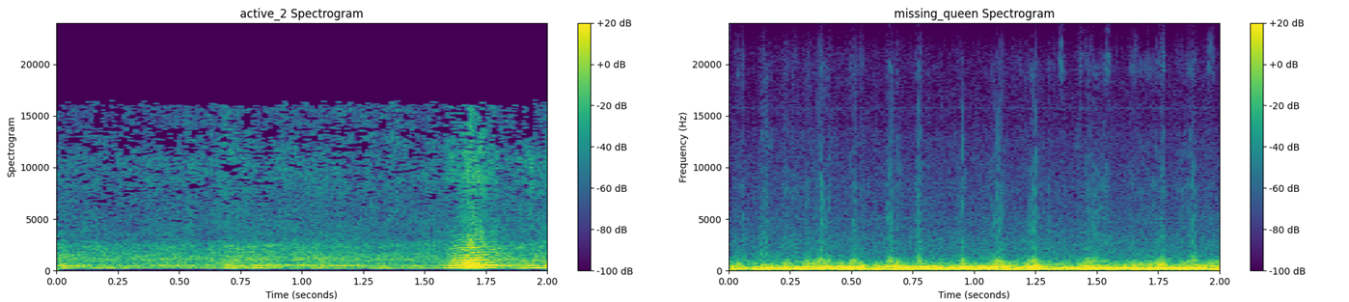
\includegraphics[width=\textwidth]{assets/cap_3/comparacion_audio.png}
    \caption{Comparación de audio.}
    \label{fig:comparacion_audio}
\end{figure}

\subsection{Características de audio}
En esta sección se describen los cálculos necesarios para extraer las características del audio de las colmenas, utilizadas en la detección de anomalías, así como su implementación en Python.

\subsubsection{Zero Crossing Rate (ZCR)}
\textit{Cálculo:}
\begin{itemize}
    \item Se divide la señal en segmentos de longitud corta.
    \item Para cada segmento, se cuenta la cantidad de veces que la señal cruza el eje cero (ZCR).
    \item Se suman todas las ZCR de los segmentos y se divide por el número total de muestras para obtener la tasa promedio.
\end{itemize}
Para lograr esto, es necesario iterar sobre cada uno de los valores de la señal y contar los cruces de cero. El código en Python para calcular ZCR sobre un segmento ya recortado es el siguiente:
\begin{lstlisting}[language=Python, label={lst:zcr_code}, caption={Cálculo de Zero Crossing Rate (ZCR) en Python}]
import numpy as np
def zero_crossing_rate(signal):
    signed_signal = np.sign(signal) # Convierte la señal a valores -1 o 1 basandose en el signo de cada muestra, -1 si la muestra es negativa, 1 si es positiva Ej: [-1, 1, -1, 1, 1]
    diff_signal = np.diff(signed_signal) # Calcular la diferencia entre muestras consecutivas Ej: [2, -2, 2, 0]
    abs_diff_signal = np.abs(diff_signal) # Tomar el valor absoluto de las diferencias Ej: [2, 2, 2, 0]
    sum_zcr = np.sum(abs_diff_signal) # Sumar las diferencias absolutas Ej: 2 + 2 + 2 + 0 = 6
    zcr = sum_zcr / (2 * len(signal)) # Dividir por el doble del numero de muestras para obtener la tasa promedio, se multiplica por 2 porque se considera la diferencia entre 1 y -1 (2) como un cruce de 0, Ej: 6 / (2 * 5) = 0.6
    return zcr
\end{lstlisting}

Sin embargo, actualmente, librerías de Python como \texttt{librosa} \cite{mcfee_librosa_2025} ya cuentan con una función para calcular el ZCR, por lo que no es necesario implementar el código desde cero. El \autoref{lst:zcr_librosa_code} muestra cómo utilizar la función:

\[
    \texttt{librosa.feature.zero\_crossing\_rate}
\]

\begin{lstlisting}[language=Python, label={lst:zcr_librosa_code}, caption={Cálculo de Zero Crossing Rate (ZCR) utilizando librosa en Python}]
import librosa
def calculate_zcr(signal, sr):
    zcr = librosa.feature.zero_crossing_rate(signal, frame_length=2048, hop_length=512)
    return zcr
\end{lstlisting}

De esta manera, se obtiene una matriz que contiene una fila por cada canal de audio, dando como resultado una matriz de forma $(1, N)$ para audios monoaurales, o $(2, N)$ para audios estéreo, donde $N$ es el número de frames calculados. Cabe destacar que, por defecto, Librosa convierte el audio a mono, por lo que es necesario desactivar esta opción para conservar múltiples canales.

Para obtener el ZCR de una señal de audio estéreo se debe de especificar el parámetro \texttt{mono=False} al llamar a la función \texttt{librosa.feature.zero\_crossing\_rate}, como se especifica en el \autoref{lst:zcr_librosa_stereo_code}:

\begin{lstlisting}[language=Python, label={lst:zcr_librosa_stereo_code}, caption={Cálculo de Zero Crossing Rate (ZCR) para audio estéreo utilizando librosa en Python}]
import librosa
def calculate_zcr_stereo(signal, sr):
    zcr = librosa.feature.zero_crossing_rate(signal, frame_length=2048, hop_length=512, mono=False)
    return zcr
\end{lstlisting}

\subsubsection{Energía}
\textit{Cálculo:} La energía de una señal discreta se calcula como la suma de los cuadrados de sus muestras. Matemáticamente, se expresa como:
\[
    \text{Energía} = \sum_{n=1}^{N} x[n]^2
\]
Donde $x[n]$ representa el valor de la señal en el instante $n$, y $N$ es el número total de muestras consideradas. Esta métrica refleja la cantidad total de potencia contenida en la señal durante el intervalo de análisis, siendo útil para detectar eventos de alta intensidad en señales de audio.

Para calcular la energía de un segmento de audio en Python, se puede utilizar el siguiente código:
\begin{lstlisting}[language=Python, label={lst:energy_code}, caption={Cálculo de energía en Python}]
import numpy as np
def calculate_energy(signal: np.ndarray) -> float:
    energy = np.sum(signal**2)  # Suma de los cuadrados de las muestras
    return energy
\end{lstlisting}

De la misma manera, la librería \texttt{librosa} \cite{mcfee_librosa_2025} permite calcular la energía por frames. El \autoref{lst:energy_librosa_code} muestra cómo hacerlo:
\begin{lstlisting}[language=Python, label={lst:energy_librosa_code}, caption={Cálculo de energía por tramas utilizando librosa}]
import librosa
import numpy as np

def calculate_frame_energy(signal: np.ndarray, frame_length: int = 2048, hop_length: int = 512) -> np.ndarray:
    frames = librosa.util.frame(signal, frame_length=frame_length, hop_length=hop_length)
    energy = np.sum(frames**2, axis=0)
    return energy  # np.ndarray con energía por trama
\end{lstlisting}

\subsubsection{RMS (Root Mean Square) de energía}

\textit{Cálculo:} El valor RMS se calcula como la raíz cuadrada del promedio de los cuadrados de las muestras de la señal. Matemáticamente, se expresa como:
\[
    \text{RMS} = \sqrt{ \frac{1}{N} \sum_{n=1}^{N} x[n]^2 }
\]
Donde \( x[n] \) es el valor de la señal en el instante \( n \), y \( N \) es el número total de muestras consideradas. El valor RMS proporciona una medida de la magnitud efectiva de la señal, siendo especialmente útil para comparar niveles de energía entre diferentes segmentos de audio.

Para calcular el RMS de un segmento de audio en Python, se puede utilizar el siguiente código:

\begin{lstlisting}[language=Python, label={lst:rms_manual_code}, caption={Cálculo de RMS por tramas sin librosa}]
import numpy as np

def calculate_rms_manual(signal: np.ndarray, frame_length: int = 2048, hop_length: int = 512) -> np.ndarray:
    rms = []
    for i in range(0, len(signal) - frame_length + 1, hop_length):
        frame = signal[i:i + frame_length]
        rms_value = np.sqrt(np.mean(frame**2))
        rms.append(rms_value)
    return np.array(rms)  # np.ndarray con valores RMS por trama
\end{lstlisting}

La libreria \texttt{librosa} \cite{mcfee_librosa_2025} también proporciona una función para calcular el RMS de una señal de audio. El \autoref{lst:rms_librosa_code} muestra cómo utilizar esta función para obtener el RMS por frames:

\begin{lstlisting}[language=Python, label={lst:rms_librosa_code}, caption={Cálculo de RMS utilizando librosa}]
import librosa
import numpy as np

def calculate_rms_librosa(signal: np.ndarray, frame_length: int = 2048, hop_length: int = 512) -> np.ndarray:
    rms = librosa.feature.rms(y=signal, frame_length=frame_length, hop_length=hop_length)[0]
    return rms  # np.ndarray con valores RMS por trama
\end{lstlisting}

\subsubsection{Entropía de energía}

\textit{Cálculo:} El frame de la señal se divide en $k$ sub-bandas de igual tamaño. Para cada sub-banda se calcula su energía local, y luego se normalizan estas energías para obtener una distribución de probabilidad \( \{p_i\} \), donde \( p_i \) representa la proporción de energía en la sub-banda \( i \) respecto a la energía total del frame. Finalmente, se aplica la fórmula de entropía:

\[
    H = -\sum_{i=1}^{k} p_i \log_2 p_i
\]

Este valor mide la dispersión o aleatoriedad de la energía dentro del frame. Un valor alto indica que la energía está distribuida uniformemente entre las sub-bandas (mayor desorden), mientras que un valor bajo sugiere concentración de energía en pocas bandas (mayor estructura o tono definido).

Para calcular la entropía de energía de un segmento de audio en Python, se puede utilizar el siguiente código:

\begin{lstlisting}[language=Python, label={lst:entropy_energy_librosa_code}, caption={Cálculo de entropía de energía utilizando librosa en Python}]
import librosa
import numpy as np
def calculate_entropy_energy_librosa(signal, sr, num_bands=10):
    # Calcular la energía por frame
    energy = librosa.feature.rms(signal, frame_length=2048, hop_length=512)[0]
    # Dividir la energía en sub-bandas
    band_size = int(np.ceil(len(energy) / num_bands))
    band_energy = np.array([np.sum(energy[i*band_size:(i+1)*band_size]) for i in range(num_bands)])
    # Normalizar las energías para obtener una distribución de probabilidad
    total_energy = np.sum(band_energy)
    p = band_energy / (total_energy + 1e-10)
    # Calcular la entropía
    entropy = -np.sum(p * np.log2(p + 1e-10))
    return entropy

\end{lstlisting}

Para el caso de



\subsubsection{Centroide espectral}

\textit{Cálculo:}

\[
    \text{Centroide} = \frac{\sum_{k=1}^{K} f_k \cdot |X(f_k)|}{\sum_{k=1}^{K} |X(f_k)|}
\]

\textit{Donde:}

\begin{itemize}
    \item \( f_k \): frecuencia correspondiente al bin \( k \).
    \item \( |X(f_k)| \): magnitud espectral en \( f_k \).
\end{itemize}

El centroide espectral representa el “centro de masa” del espectro de magnitudes y se asocia con la percepción de brillo del sonido. Valores más altos indican mayor presencia de componentes de alta frecuencia.


\subsubsection{Dispersión espectral}
\textit{Cálculo:} $\text{Spread} = \sqrt{\frac{\sum |X(f_k)|(f_k - \text{Centroide})^2}{\sum |X(f_k)|}}$

\subsubsection{Entropía espectral}
\textit{Cálculo:} Se normaliza el espectro a una distribución de probabilidad y se aplica: $H = -\sum p_k \log_2 p_k$

\subsubsection{Flujo espectral}
\textit{Cálculo:} $\text{Flux} = \sum_k \left( |X_{t}(f_k)| - |X_{t-1}(f_k)| \right)^2$, comparando magnitudes espectrales entre frames $t$ y $t-1$.

\subsubsection{Rolloff espectral}
\textit{Cálculo:} Se busca la frecuencia $f_r$ tal que $\sum_{f=0}^{f_r} |X(f)| = 0.85 \cdot \sum_{f=0}^{f_{max}} |X(f)|$

\subsubsection{MFCC (1 a 13)}
\textit{Cálculo:} Se aplica una ventana a la señal, luego FFT → banco de filtros en escala Mel → logaritmo → Transformada Discreta del Coseno (DCT). Se conservan los primeros 13 coeficientes.